\documentclass[unicode,9pt,a4paper,oneside,numbers=endperiod,openany]{scrartcl}

\renewcommand{\thesubsection}{\arabic{subsection}}

\usepackage{ifthen}
\usepackage[utf8]{inputenc}
\usepackage{graphics}
\usepackage{graphicx}
\usepackage{hyperref}

\pagestyle{plain}
\voffset -20mm
\oddsidemargin  0mm
\evensidemargin -11mm
\marginparwidth 2cm
\marginparsep 0pt
\topmargin 0mm
\headheight 0pt
\headsep 0pt
\topskip 0pt
\textheight 255mm
\textwidth 165mm

\newcommand{\duedate} {}
\newcommand{\setduedate}[1]{%
  \renewcommand\duedate {\textbf{Due date:}~ #1}}
\newcommand\isassignment {false}
\newcommand{\setassignment}{\renewcommand\isassignment {true}}
\newcommand{\ifassignment}[1]{\ifthenelse{\boolean{\isassignment}}{#1}{}}
\newcommand{\ifnotassignment}[1]{\ifthenelse{\boolean{\isassignment}}{}{#1}}


\newcommand{\punkte}[1]{\hspace{1ex}\emph{\mdseries\hfill(#1~\ifcase#1{Points}\or{Points}\else{Points}\fi)}}


\newcommand\serieheader[6]{
\thispagestyle{empty}%
\begin{flushleft}
  
\includegraphics[width=0.3\textwidth]{CI_logo}
\end{flushleft}
\noindent%
{\large\ignorespaces{\textbf{#1}}\hspace{\fill}\ignorespaces{ \textbf{#2}}}\\ \\%
{\large\ignorespaces #3 \hspace{\fill}\ignorespaces #4}\\
% \noindent%
% \bigskip
% \hrule\par\bigskip\noindent%
{\ignorespaces {\Large{\textbf{#5}}}
\hspace{\fill}\ignorespaces \large \ifthenelse{\boolean{\isassignment}}{\duedate}{#6}}
\hrule\par\noindent%  \linebreak
}

\makeatletter
\def\enumerateMod{\ifnum \@enumdepth >3 \@toodeep\else
    \advance\@enumdepth \@ne
    \edef\@enumctr{enum\romannumeral\the\@enumdepth}\list
    {\csname label\@enumctr\endcsname}{\usecounter
      {\@enumctr}%%%? the following differs from "enumerate"
      \topsep0pt%
      \partopsep0pt%
      \itemsep0pt%
      \def\makelabel##1{\hss\llap{##1}}}\fi}
\let\endenumerateMod =\endlist
\makeatother




\usepackage{textcomp}





\usepackage{amssymb}
\begin{document}


\setassignment
\setduedate{Wednesday, 27 November 2024, 11:59 PM}

\serieheader{Information Retrieval}{2024}{\textbf{Student:} Costanza Rodiguez Gavazzi, Agnese Zamboni, Davide Frova}{}
\newline


\section{Overview}
The Information Retrieval project is advancing according to plan. The responsibilities have been allocated among three team members, each concentrating on a separate part of the project.

\section{Frontend Design and Implementation}
Davide is responsible for the frontend design and implementation. The initial design research and UI mockup creation have been completed using Figma. The next steps involve implementing the design using Next.js.
The design aims to be minimalistic and user-friendly.
The current prototype contains simple search bar with the iconic search button, the length of the bar is not too short to incentivize the user to type longer queries.
A logo representing the project will be placed above the search bar, this will aim to give the user a sense of the project's identity.
Under the search bar we have the three pill shaped filter dropdowns, we identified as possible filters: the charity 'theme', the 'location' and the last filter is still to be decided.
After entering the query the user will be presented with a list of cards cotaining various informations about the charities, such as the name, the logo and a "google snippet" like description with highlighted keywords.
There are also present the 'thumb up' and 'thumb down' buttons to allow the user to give feedback on the results, this will re-run the query with the feedback in mind.
\\Here are some screenshots of the current design:
\begin{figure}[h]
    \centering
    \begin{minipage}{0.45\textwidth}
        \centering
        
\includegraphics[width=\textwidth]{fig/mockup1.png}
        \caption{Mockup Search Page}
    \end{minipage}\hfill
    \begin{minipage}{0.45\textwidth}
        \centering
        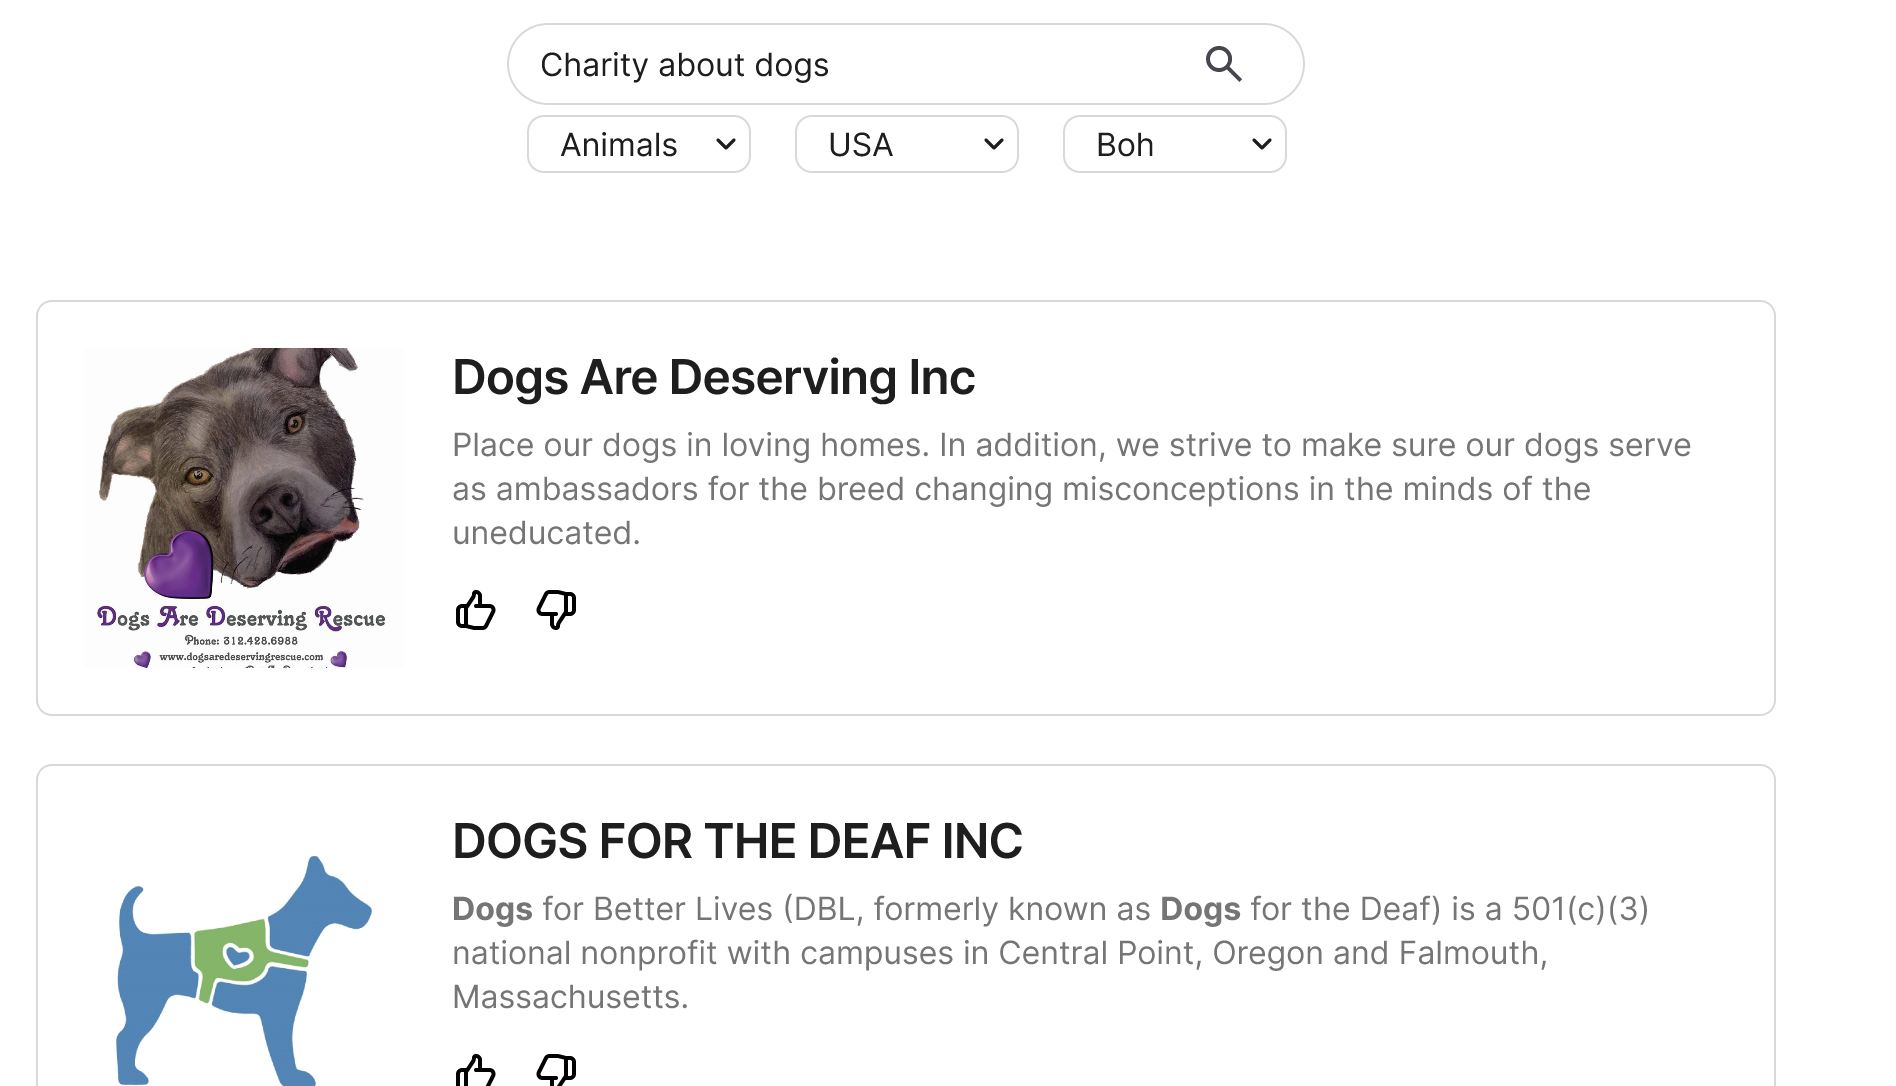
\includegraphics[width=\textwidth]{fig/mockup2.png}
        \caption{Mockup Results Browsing}
    \end{minipage}
\end{figure}

\section{Data Collection and Processing}
We built data processing systems for two major charity platforms - Global Giving and Charity Navigator. Each required a different approach due to how their data is made available. \\
\hfill \\

For Global Giving, we used their API to download the available data in XML format. Rather than scraping their website, we wrote a parser to extract information from this structured data file. The system processes several types of information about each organization:

\begin{itemize}
    \item Basic details like their name and location
    \item Operational metrics (active and total projects)
    \item Mission statements and website URLs
    \item Causes they work on ("themes")
    \item Countries where they operate
\end{itemize}

After getting this data, we enhanced it with additional geographical information using pycountry and pycountry\_convert libraries. This let us add continental classifications based on each organization's headquarters location. We also improved the data structure - renaming fields to be consistent with the data fro and reorganizing the information about operational territories to make it more useful for analysis.

The Charity Navigator system needed a different approach since they have a modern API. We used their GraphQL API instead of a regular REST API because it's more efficient - we can specify exactly what data we want, avoid making multiple calls, and handle nested data better. The system can handle large amounts of data, processing up to 10,000 records in small batches to avoid overwhelming their server.
One of our biggest technical challenges was automatically finding logos on charity websites. We built a system that uses multiple approaches to find the right logo:

First, it looks through the webpage's structure for anything marked as a logo
Then it checks special webpage tags that often contain logos
It also looks for icon links and any images that might be logos
Finally, it carefully checks each potential logo to make sure it's not picking up the wrong things (like menu icons)

We used several standard Python libraries to build these systems. BeautifulSoup handles the messy HTML we sometimes get from websites. The requests library manages all our web connections. We used pycountry for standardizing country names and codes.
All the data gets saved in JSON format. We chose JSON because:

\begin{itemize}
    \item It works with pretty much any system
    \item It's easy to read when debugging
    \item It handles nested data well
    \item Other tools can easily work with it
\end{itemize}

We made sure the systems could handle problems gracefully. Instead of crashing when something goes wrong, they skip the problem and keep going. This means we get as much data as possible while keeping it accurate.
This whole setup gives us a solid foundation for analyzing charitable organizations. The systems are built to:

\begin{itemize}
    \item Keep the data high quality and complete
    \item Work reliably even when things go wrong
    \item Handle large amounts of data efficiently
    \item Output data in a standard format
    \item Allow for future improvements
\end{itemize}

These choices mean we can analyze organizations in detail - looking at where they work, what they focus on, and how they operate, while keeping the systems maintainable and reliable.

\section{Backend and Indexing/Retrieval}
Agnese is focusing on the backend and indexing/retrieval part.
We have chosen PyTerrier for indexing and searching the data, and FastAPI to create a simple Python backend that will interface with PyTerrier.
The necessary endpoints for the frontend-backend communication are being defined.
An draft of the main endpoint comprehends parameters for the user query, the filters and the feedback on a result.
\begin{verbatim}
GET /search?q=userQuery&filters=filter1,filter2,filter3&feedback={docId:123,score:1}
\end{verbatim}

\section{User Evaluation}

\section{Appendix}


\end{document}